\chapter{Présentation de l'Organisme et Contexte du Projet}
\label{chap:contexte}

\section{Introduction}

Ce premier chapitre a pour vocation d'établir les fondations contextuelles, organisationnelles et méthodologiques du projet d'ingénierie \textbf{PMS AMH Hospitality}. Nous débuterons par une présentation détaillée du groupe d'accueil AMH Hospitality, de sa genèse, de ses activités d'exploitation de Riads à Marrakech et de son organisation interne. Nous exposerons ensuite le cadre institutionnel du stage, les missions qui nous ont été confiées ainsi que l'immersion sur le terrain hôtelier. Nous formaliserons la problématique métier et technique, les objectifs quantifiables du projet, l'étude exhaustive des exigences fonctionnelles et non fonctionnelles, pour conclure sur la méthodologie de gestion de projet Agile Scrum découpée en huit sprints de développement et sa planification temporelle par diagramme de Gantt.

\section{Présentation de l'organisme d'accueil}

\subsection{Historique et genèse du groupe}

La Figure~\ref{fig:logo_amh} illustre l'emblème et l'identité visuelle du groupe hôtelier d'accueil.

\begin{figure}[H]
\centering
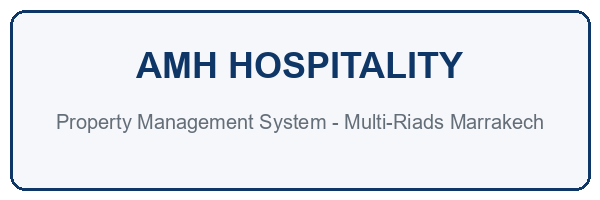
\includegraphics[width=0.7\textwidth]{figures/logo_amh.png}
\caption{Logo du groupe AMH Hospitality}
\label{fig:logo_amh}
\end{figure}

Fondé avec la vision novatrice d'allier l'art de vivre traditionnel marocain et l'excellence des standards de l'hôtellerie internationale, le groupe \textbf{AMH Hospitality} s'est rapidement imposé comme un acteur de référence dans le secteur de l'hébergement de prestige à Marrakech. Partant de la réhabilitation méticuleuse d'un premier Riad historique situé dans les ruelles séculaires de la Médina, les fondateurs du groupe ont su développer une expertise d'exception dans la transformation d'anciennes demeures patriciennes en établissements hôteliers de charme alliant architecture arabo-andalouse, confort technologique moderne et hospitalité personnalisée.

Au fil des années, AMH Hospitality a fait évoluer son modèle opérationnel vers celui d'un opérateur hôtelier multi-propriétés (\textit{Multi-Property Operator}). Cette stratégie a consisté à intégrer au sein d'une structure de management unifiée plusieurs Riads autonomes de 8 à 25 chambres (tels que le Riad Yasmine, le Riad Al Ksar et l'Éco-Lodge de la Palmeraie), tout en centralisant les fonctions de support : la tarification dynamique (\textit{Revenue Management}), les achats groupés, la communication digitale, la gestion comptable et financière, et l'infrastructure des systèmes d'information. Cette mutualisation des ressources a permis au groupe d'atteindre des taux d'occupation moyens annuels supérieurs à 82\% tout en préservant l'identité intimiste et singulière de chaque établissement.

\subsection{Activité principale et métiers}

L'activité fondamentale d'AMH Hospitality s'articule autour de la chaîne de valeur complète de l'exploitation hôtelière de luxe, structurée en trois grands domaines de compétences :

\begin{enumerate}
    \item \textbf{L'Exploitation Hôtelière et l'Expérience Client (\textit{Operations})} :
    \begin{itemize}
        \item \textit{Front Office (Accueil et Réception)} : Prise en charge individualisée des voyageurs dès leur arrivée à l'aéroport de Marrakech-Ménara, enregistrement des formalités administratives et fiches de police, remise des clés et orientation personnalisée dans la Médina ;
        \item \textit{Housekeeping (Gouvernance d'étage)} : Entretien quotidien rigoureux des suites et chambres selon des protocoles d'hygiène stricts, gestion du linge de maison traditionnel, réapprovisionnement des produits d'accueil artisanaux et inspection de conformité avant réattribution ;
        \item \textit{Conciergerie de Luxe \& Restauration} : Organisation d'excursions sur mesure dans l'Atlas et le désert d'Agafay, réservation de tables gastronomiques, et service d'une restauration marocaine raffinée (tagines mijotés, pastillas royales, thés de bienvenue).
    \end{itemize}
    \item \textbf{La Distribution Numérique et le Revenue Management} :
    \begin{itemize}
        \item Gestion multicanale des disponibilités sur les plateformes d'agences de voyage en ligne (Booking.com, Airbnb, Expedia, Agoda, TripAdvisor) et sur les canaux directs (site web officiel, réservations par messagerie et téléphone) ;
        \item Ajustement dynamique des grilles tarifaires (\textit{Dynamic Pricing}) en fonction des courbes de demande saisonnières, des grands événements culturels de Marrakech (Festival International du Film, Biennale d'art) et des durées minimales de séjour (\textit{Minimum Length of Stay}).
    \end{itemize}
    \item \textbf{Le Pilotage Financier, Comptable et Fiscal} :
    \begin{itemize}
        \item Clôtures journalières d'exploitation (\textit{Night Audit}) vérifiant la concordance entre les paiements reçus (espèces en dirhams ou devises, cartes bancaires marocaines et internationales) et les prestations consommées ;
        \item Imputation et reversement des taxes réglementaires marocaines obligatoires : la Taxe sur la Valeur Ajoutée (TVA au taux réduit de 10\% sur l'hébergement), la Taxe de Séjour communale (TS, 25 MAD par nuitée et par personne) et la Taxe de Promotion Touristique (TPT, 12 MAD par nuitée et par personne) ;
        \item Consolidation comptable multi-établissements et production des états financiers mensuels pour la direction générale.
    \end{itemize}
\end{enumerate}

\subsection{Organisation structurelle du groupe}

La structure organisationnelle d'AMH Hospitality est organisée selon une gouvernance claire garantissant une coordination sans friction entre les fonctions stratégiques centrales et les équipes opérationnelles déployées sur site. L'organisation se subdivise en quatre directions :

\begin{itemize}
    \item \textbf{Direction Générale (DG)} : Impulse la vision stratégique, pilote les investissements immobiliers et veille au respect de l'identité de marque du groupe ;
    \item \textbf{Direction des Opérations Hôtelières (DOH)} : Supervise les directeurs de Riads, coordonne les gouvernantes générales et garantit le maintien des plus hauts standards de satisfaction client ;
    \item \textbf{Direction Administrative et Financière (DAF)} : Contrôle la rentabilité opérationnelle, supervise la gestion de trésorerie, valide les audits comptables et gère les ressources humaines ;
    \item \textbf{Pôle Systèmes d'Information et Transformation Digitale (SI)} : Conçoit, déploie et administre l'ensemble de l'écosystème logiciel et de l'infrastructure réseau et cloud du groupe.
\end{itemize}

\subsection{Département d'accueil : Pôle Systèmes d'Information}

Notre stage d'ingénierie a été réalisé au sein du \textbf{Pôle Systèmes d'Information et Transformation Digitale}. Ce département a pour mission d'internaliser l'expertise technologique au sein d'AMH Hospitality, afin de s'affranchir de la dépendance envers des solutions logicielles tierces propriétaires souvent onéreuses, rigides et inadaptées aux spécificités fiscales et opérationnelles des Riads marocains.

Sous la responsabilité directe du Lead Architect (notre encadrant professionnel), le pôle SI est en charge de :
\begin{itemize}
    \item L'urbanisation des architectures logicielles et l'orchestration des conteneurs microservices ;
    \item La sécurisation des identités numériques, des transactions financières et des données personnelles des voyageurs (conformité RGPD et loi marocaine 09-08) ;
    \item L'industrialisation des chaînes d'intégration et de déploiement continus (CI/CD) ;
    \item L'assistance technique et l'accompagnement au changement des équipes de réception et de gouvernance d'étage.
\end{itemize}

\section{Présentation du stage}

\subsection{Cadre académique et institutionnel}

Ce projet s'inscrit dans le cadre du \textbf{Projet de Fin d'Année (PFA) / Stage d'Ingénieur}, composante majeure du cursus de formation d'ingénieurs à l'École Marocaine des Sciences de l'Ingénieur (EMSI Marrakech), membre du réseau international Honoris United Universities. Ce stage professionnalisant constitue une opportunité d'appliquer des compétences théoriques et techniques avancées à la résolution d'une problématique industrielle réelle, complexe et soumise à de fortes exigences de disponibilité, de cohérence transactionnelle et de scalabilité.

\subsection{Fiche signalétique du stage}

Le Tableau~\ref{tab:fiche_stage} récapitule l'ensemble des paramètres administratifs et d'encadrement du stage.

\begin{table}[H]
\centering
\small
\renewcommand{\arraystretch}{1.3}
\begin{tabularx}{\textwidth}{|p{4.5cm}|X|}
\hline
\textbf{Paramètre} & \textbf{Description et Caractéristiques} \\
\hline
\textbf{Établissement académique} & École Marocaine des Sciences de l'Ingénieur (EMSI Marrakech) \\
\hline
\textbf{Filière de formation} & Ingénierie Informatique \& Réseaux \\
\hline
\textbf{Organisme d'accueil} & Groupe AMH Hospitality (Marrakech, Maroc) \\
\hline
\textbf{Durée et période} & 16 semaines consécutives (Février 2026 -- Mai 2026) \\
\hline
\textbf{Lieu principal de travail} & Locaux techniques de la Direction Informatique, Marrakech \\
\hline
\textbf{Sites pilotes d'immersion} & Riad Yasmine, Riad Al Ksar (Médina de Marrakech) \\
\hline
\textbf{Encadrant professionnel} & Lead Architect (AMH Hospitality) \\
\hline
\textbf{Encadrant pédagogique} & Professeur Universitaire (EMSI Marrakech) \\
\hline
\textbf{Intitulé du projet} & Plateforme PMS Hôtelière Multi-Établissements Microservices \\
\hline
\end{tabularx}
\caption{Fiche signalétique du stage de fin d'année}
\label{tab:fiche_stage}
\end{table}

\subsection{Immersion terrain et recueil du besoin}

Afin de concevoir une solution parfaitement ancrée dans les réalités quotidiennes du métier hôtelier, notre équipe a effectué une phase d'immersion opérationnelle directe au sein des établissements pilotes du groupe à Marrakech.

La Figure~\ref{fig:pic1} et la Figure~\ref{fig:pic2} illustrent les sessions d'observation menées au comptoir de réception du Riad Yasmine.

\begin{figure}[H]
\centering
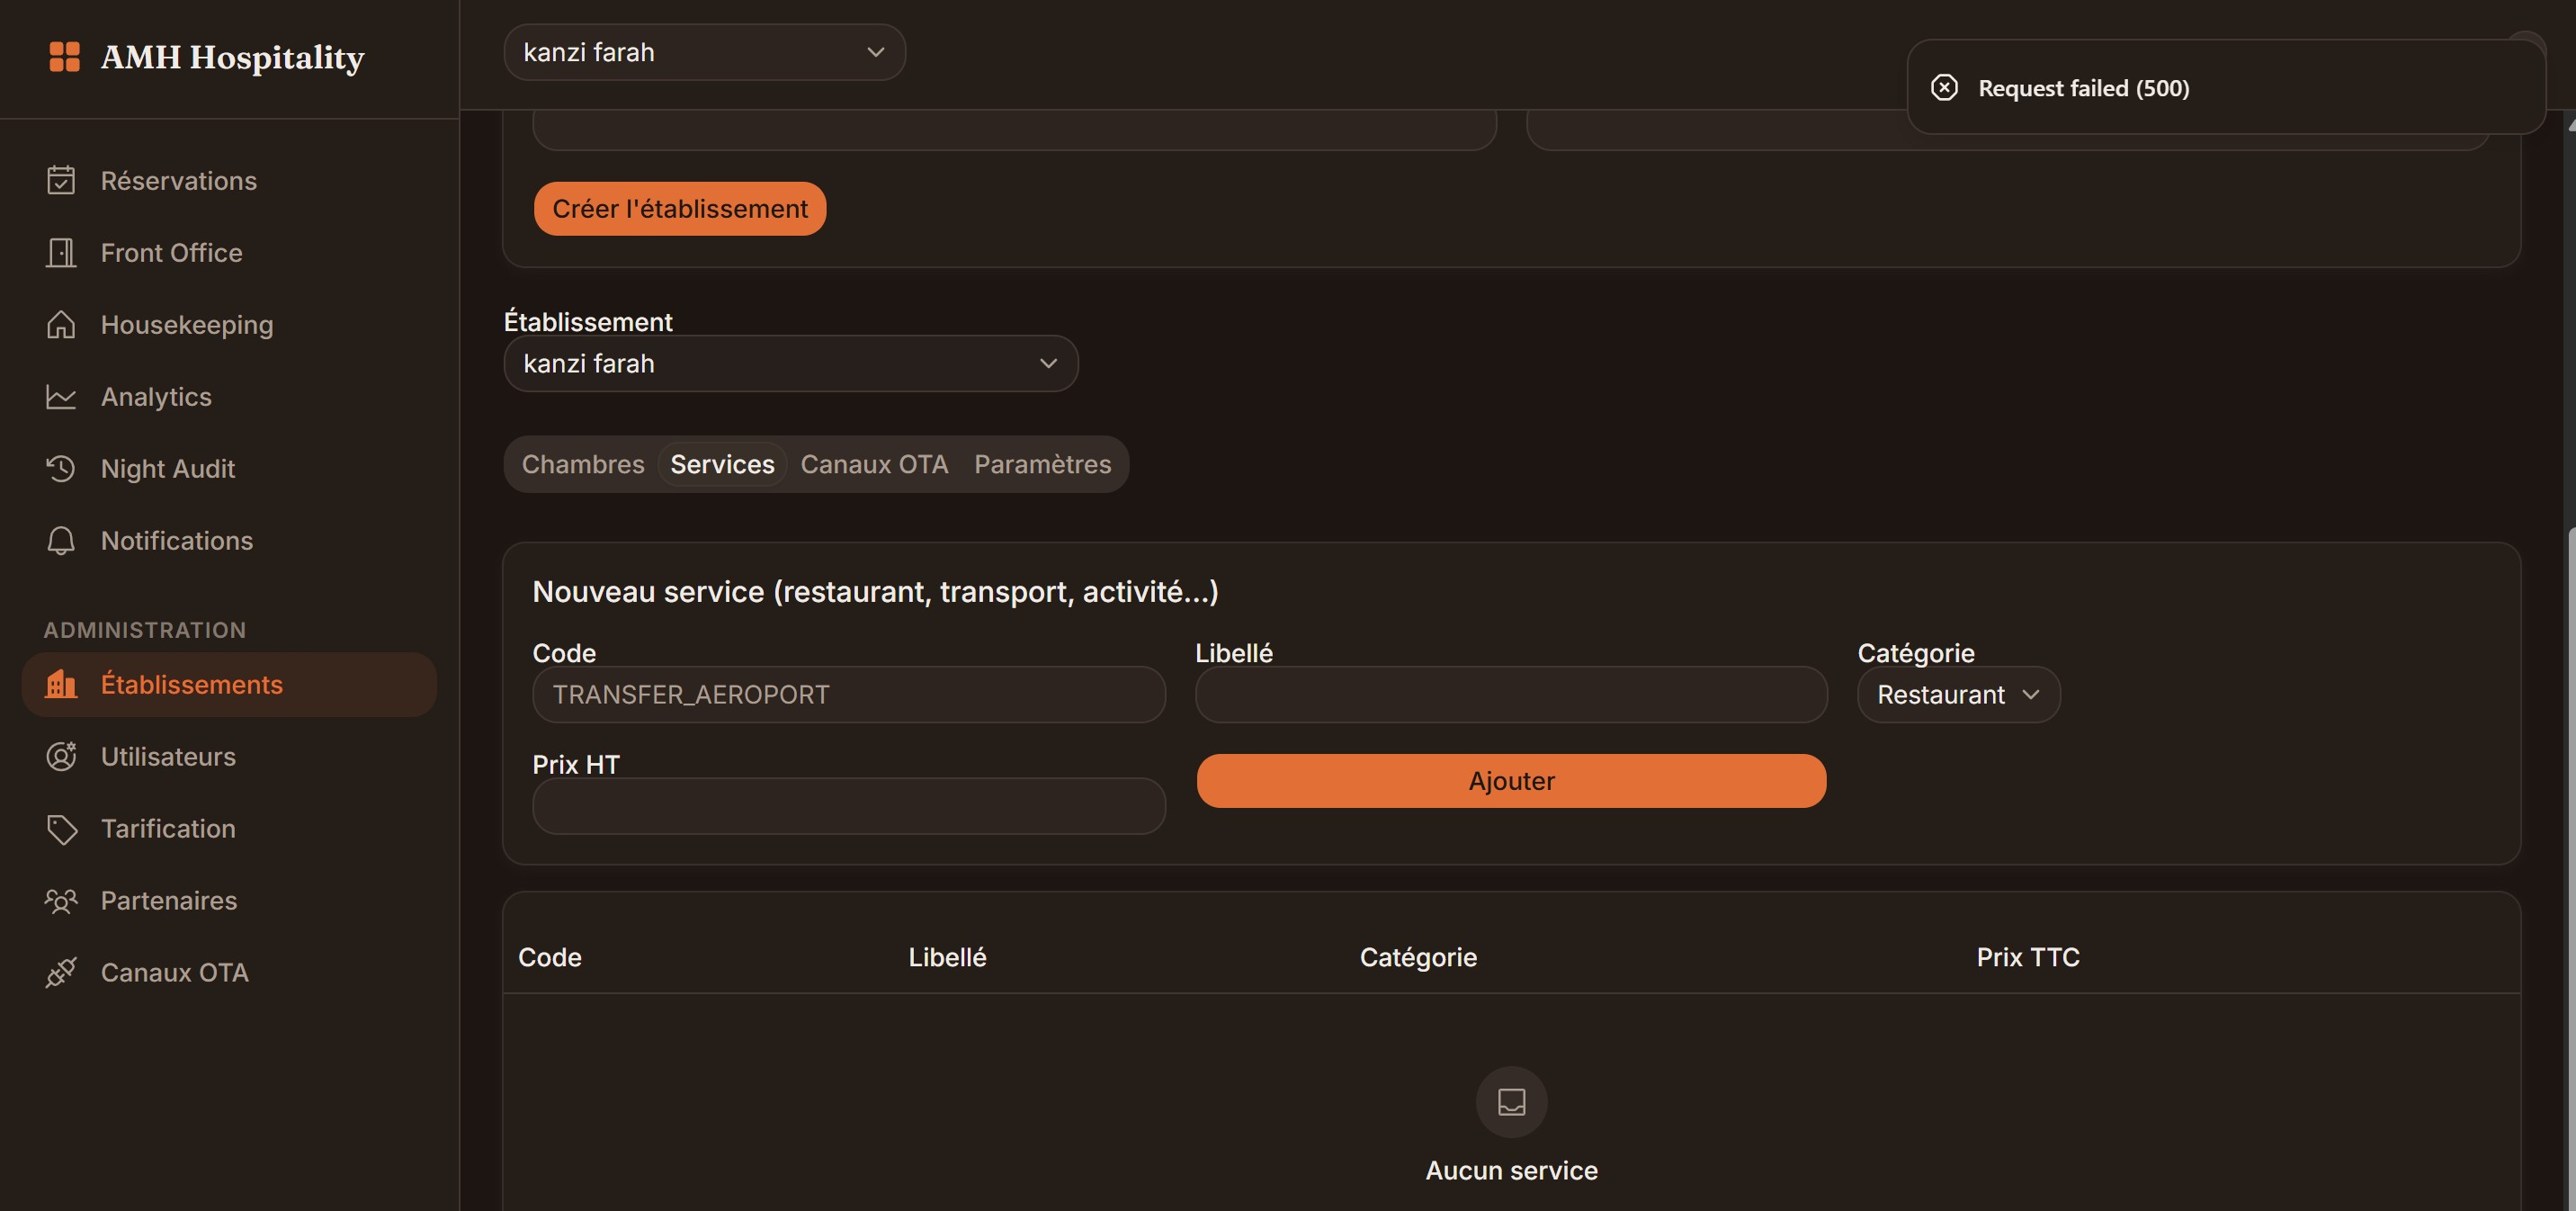
\includegraphics[width=0.75\textwidth]{figures/pic1.jpg}
\caption{Immersion opérationnelle et audit des flux d'accueil en réception}
\label{fig:pic1}
\end{figure}

\begin{figure}[H]
\centering
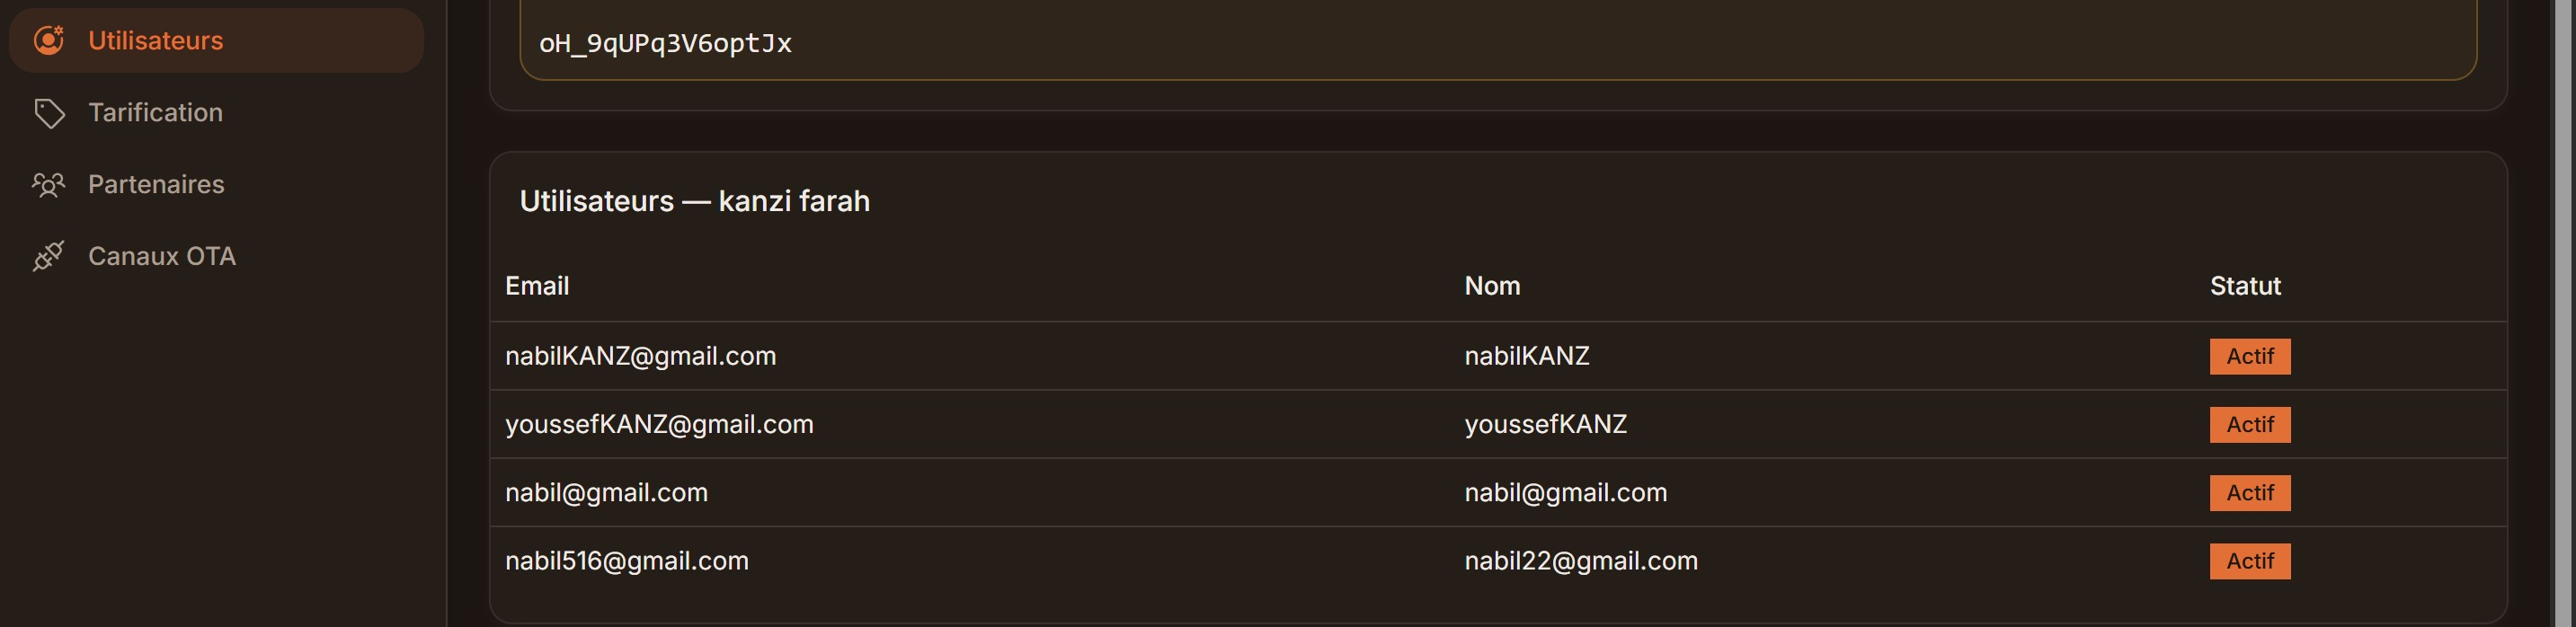
\includegraphics[width=0.75\textwidth]{figures/pic2.jpg}
\caption{Analyse des procédures manuelles de check-in et de tenue des registres}
\label{fig:pic2}
\end{figure}

Comme l'illustrent la Figure~\ref{fig:pic1} et la Figure~\ref{fig:pic2}, cette phase d'immersion a permis d'observer en direct les interactions entre les réceptionnistes et les clients, le rythme des arrivées en période de pointe, les contraintes de manipulation des pièces d'identité et la complexité des calculs fiscaux manuels.

La Figure~\ref{fig:pic3} et la Figure~\ref{fig:pic4} présentent les ateliers collaboratifs de formalisation du cahier des charges menés conjointement avec les directeurs de Riads et notre encadrant professionnel.

\begin{figure}[H]
\centering
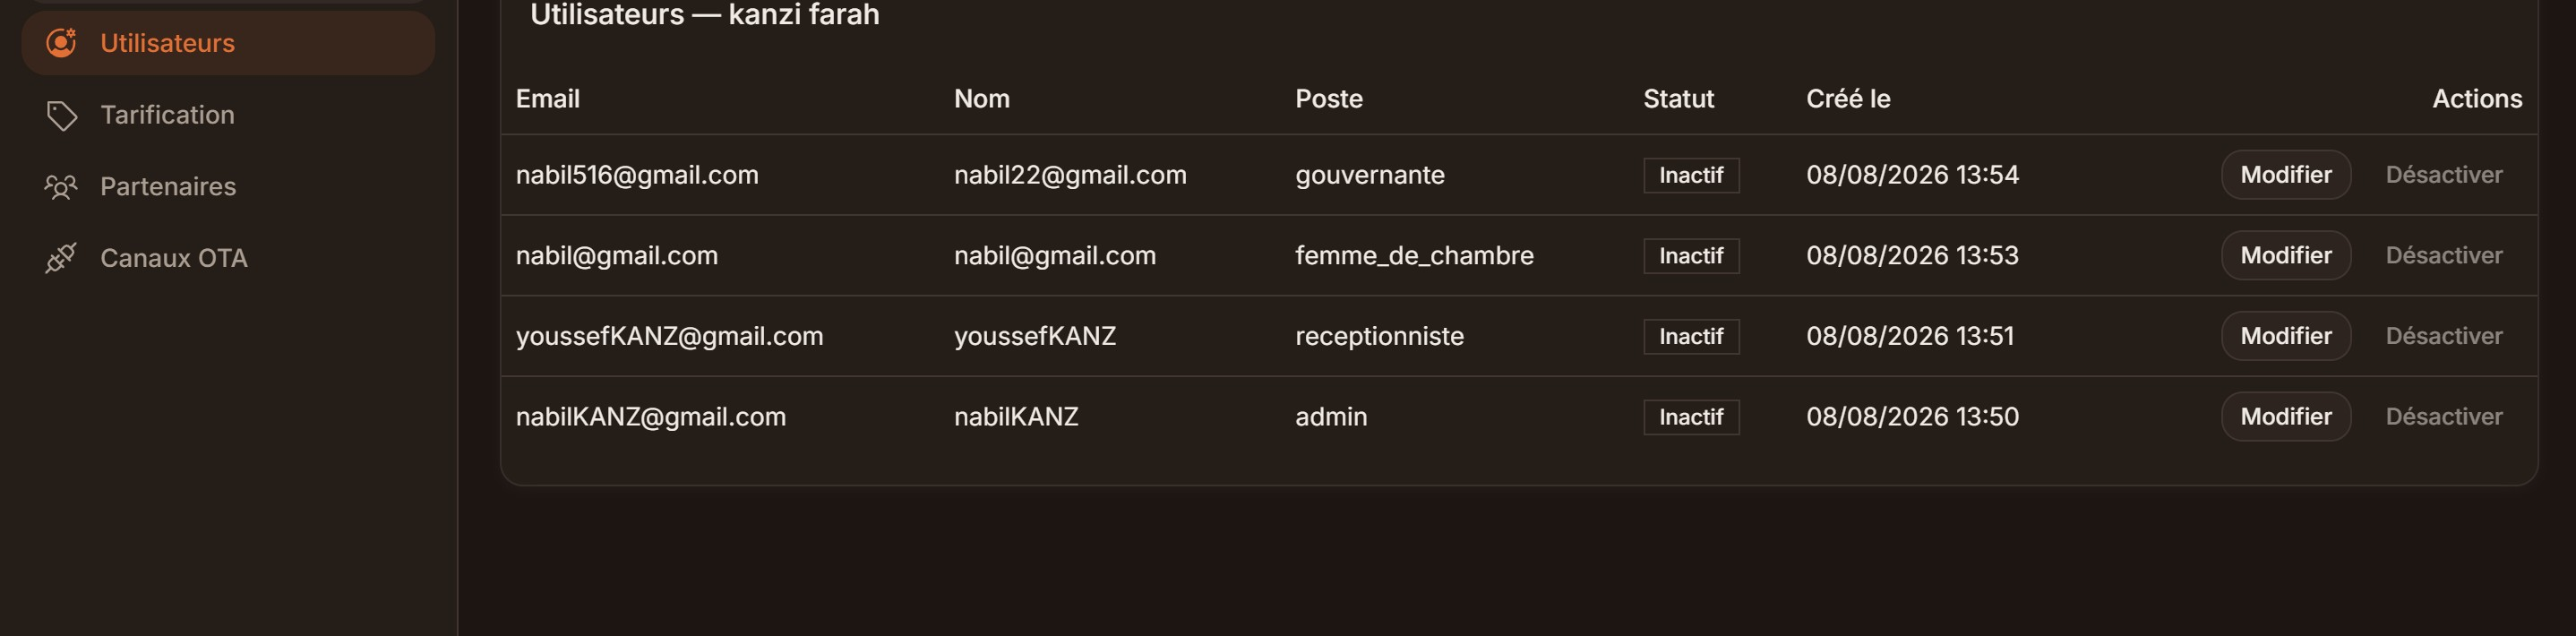
\includegraphics[width=0.75\textwidth]{figures/pic3.jpg}
\caption{Atelier de modélisation des processus métier et des règles de tarification}
\label{fig:pic3}
\end{figure}

\begin{figure}[H]
\centering
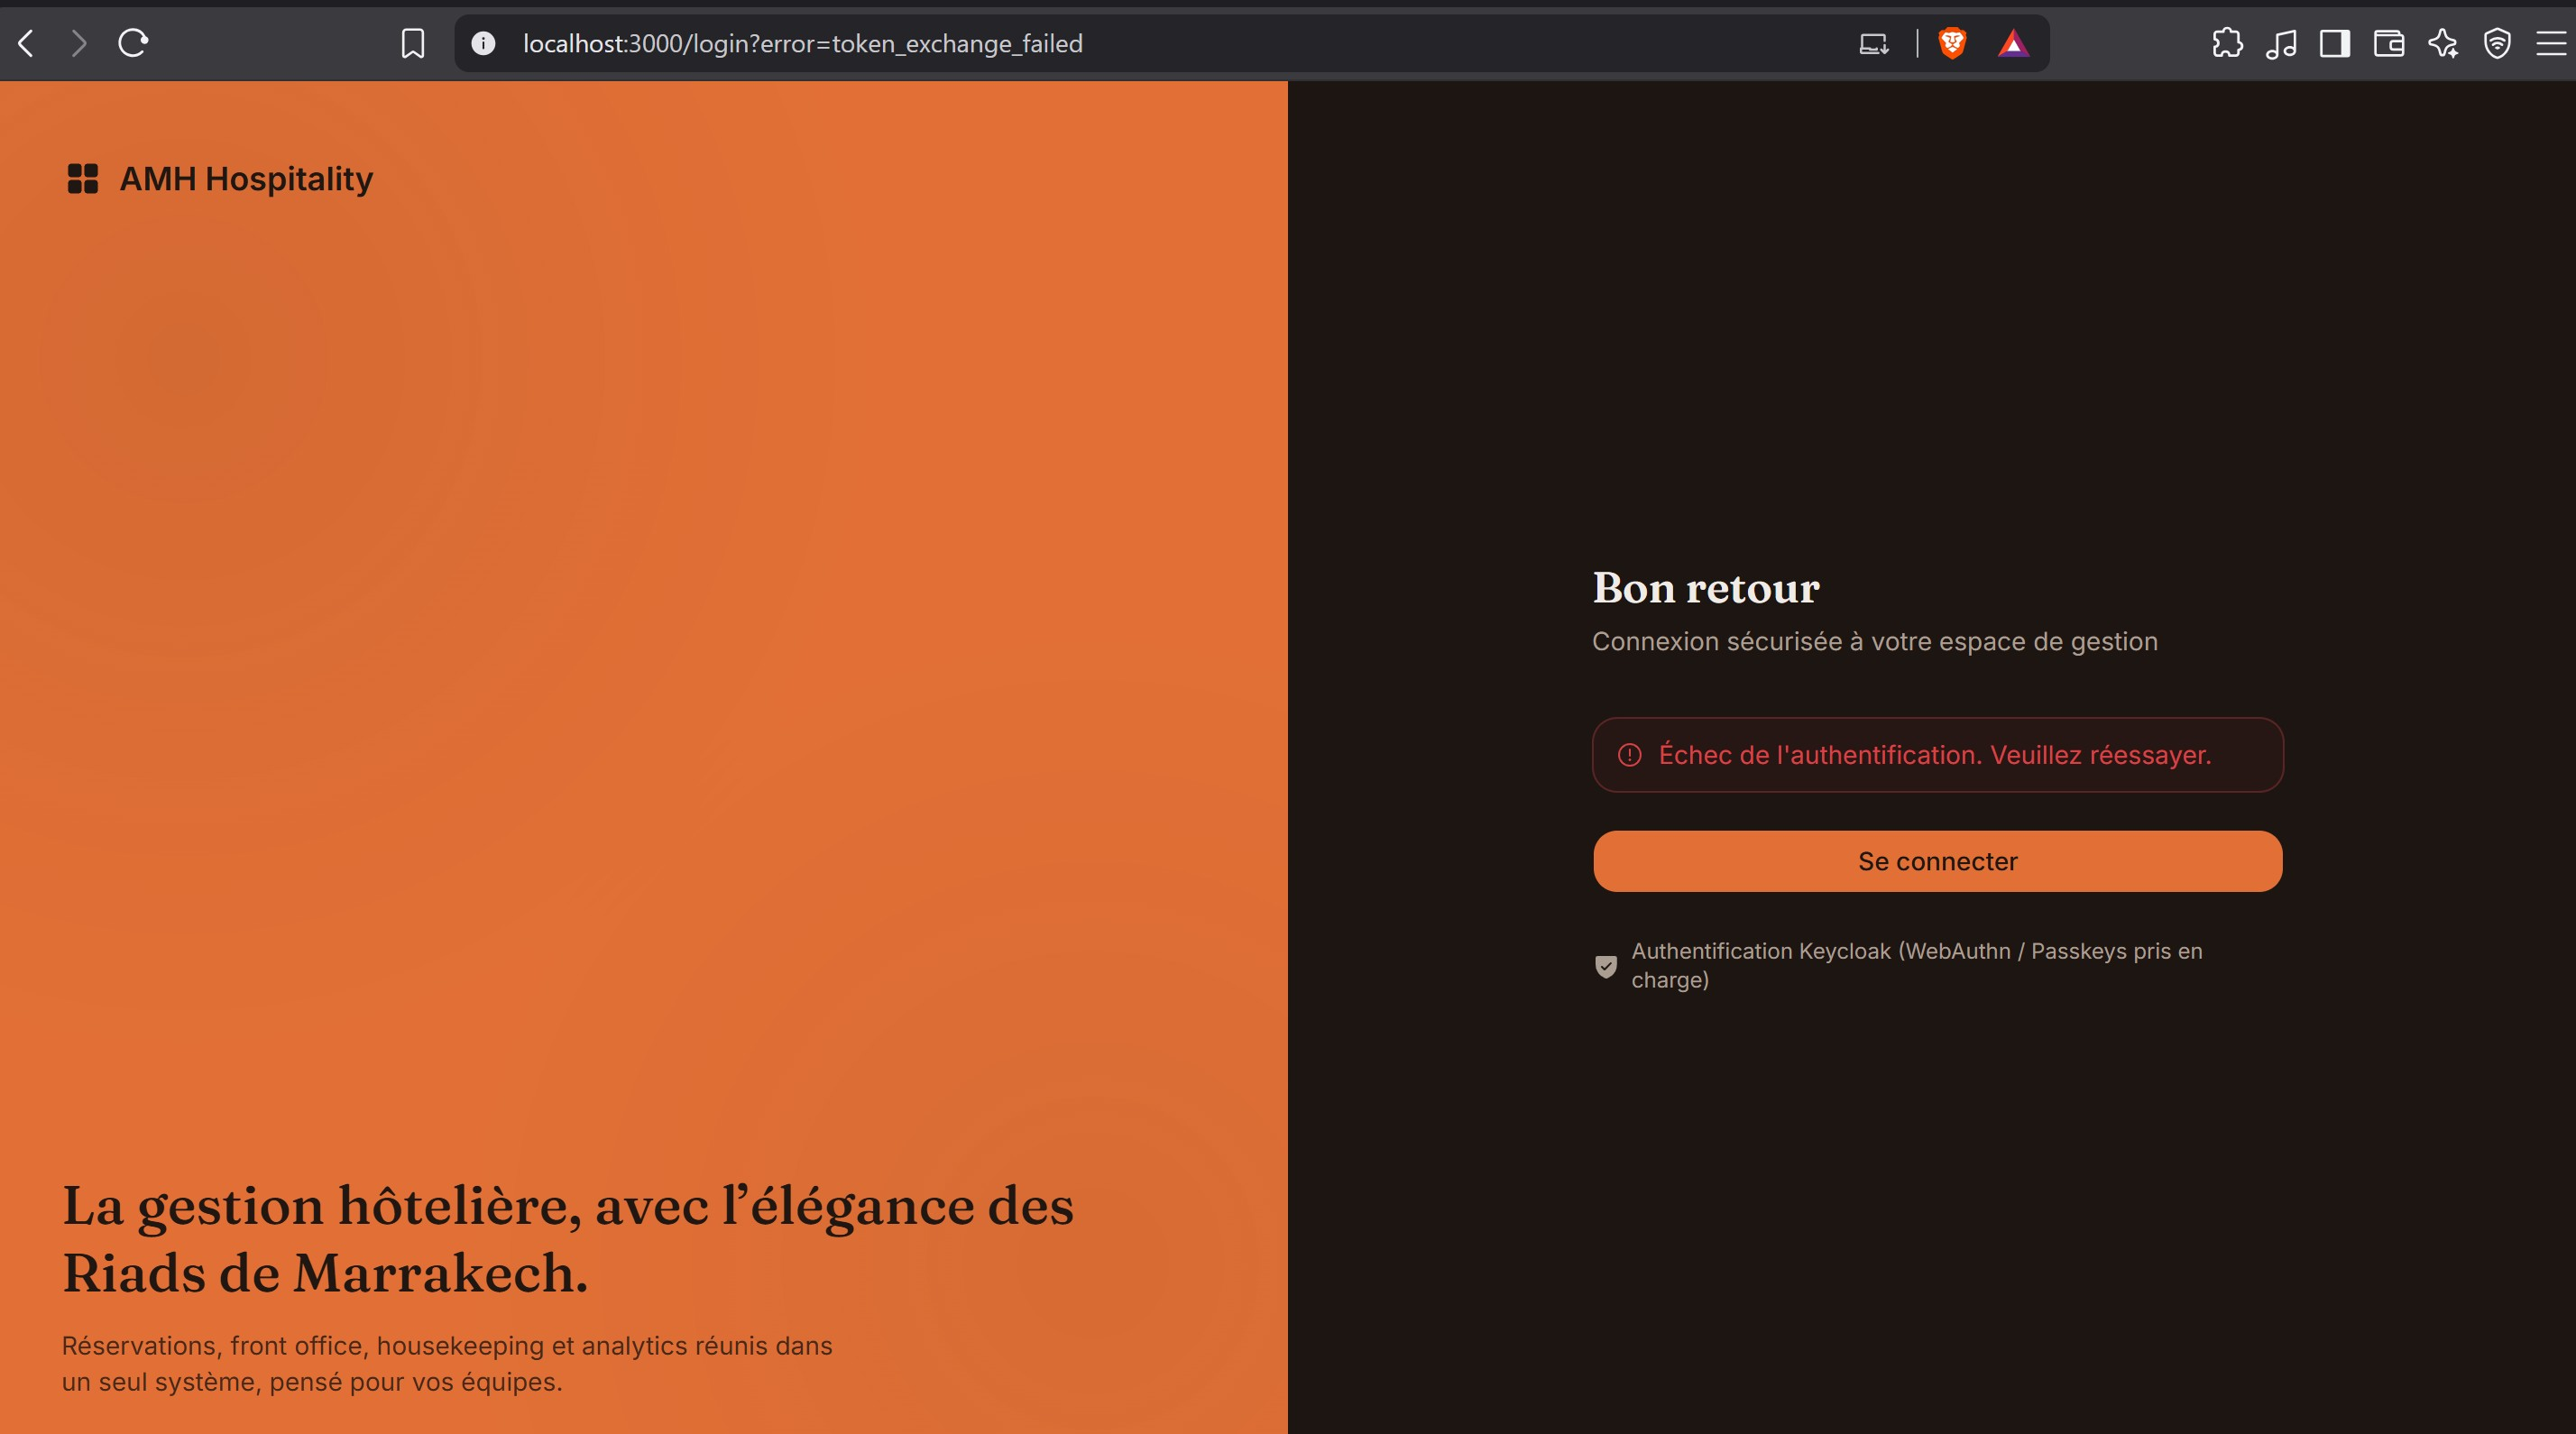
\includegraphics[width=0.75\textwidth]{figures/pic4.jpg}
\caption{Revue de cadrage technique et validation des maquettes d'interfaces}
\label{fig:pic4}
\end{figure}

La Figure~\ref{fig:pic5} et la Figure~\ref{fig:pic6} illustrent les phases de test préliminaire des prototypes déployés sur poste fixe et sur terminaux mobiles.

\begin{figure}[H]
\centering
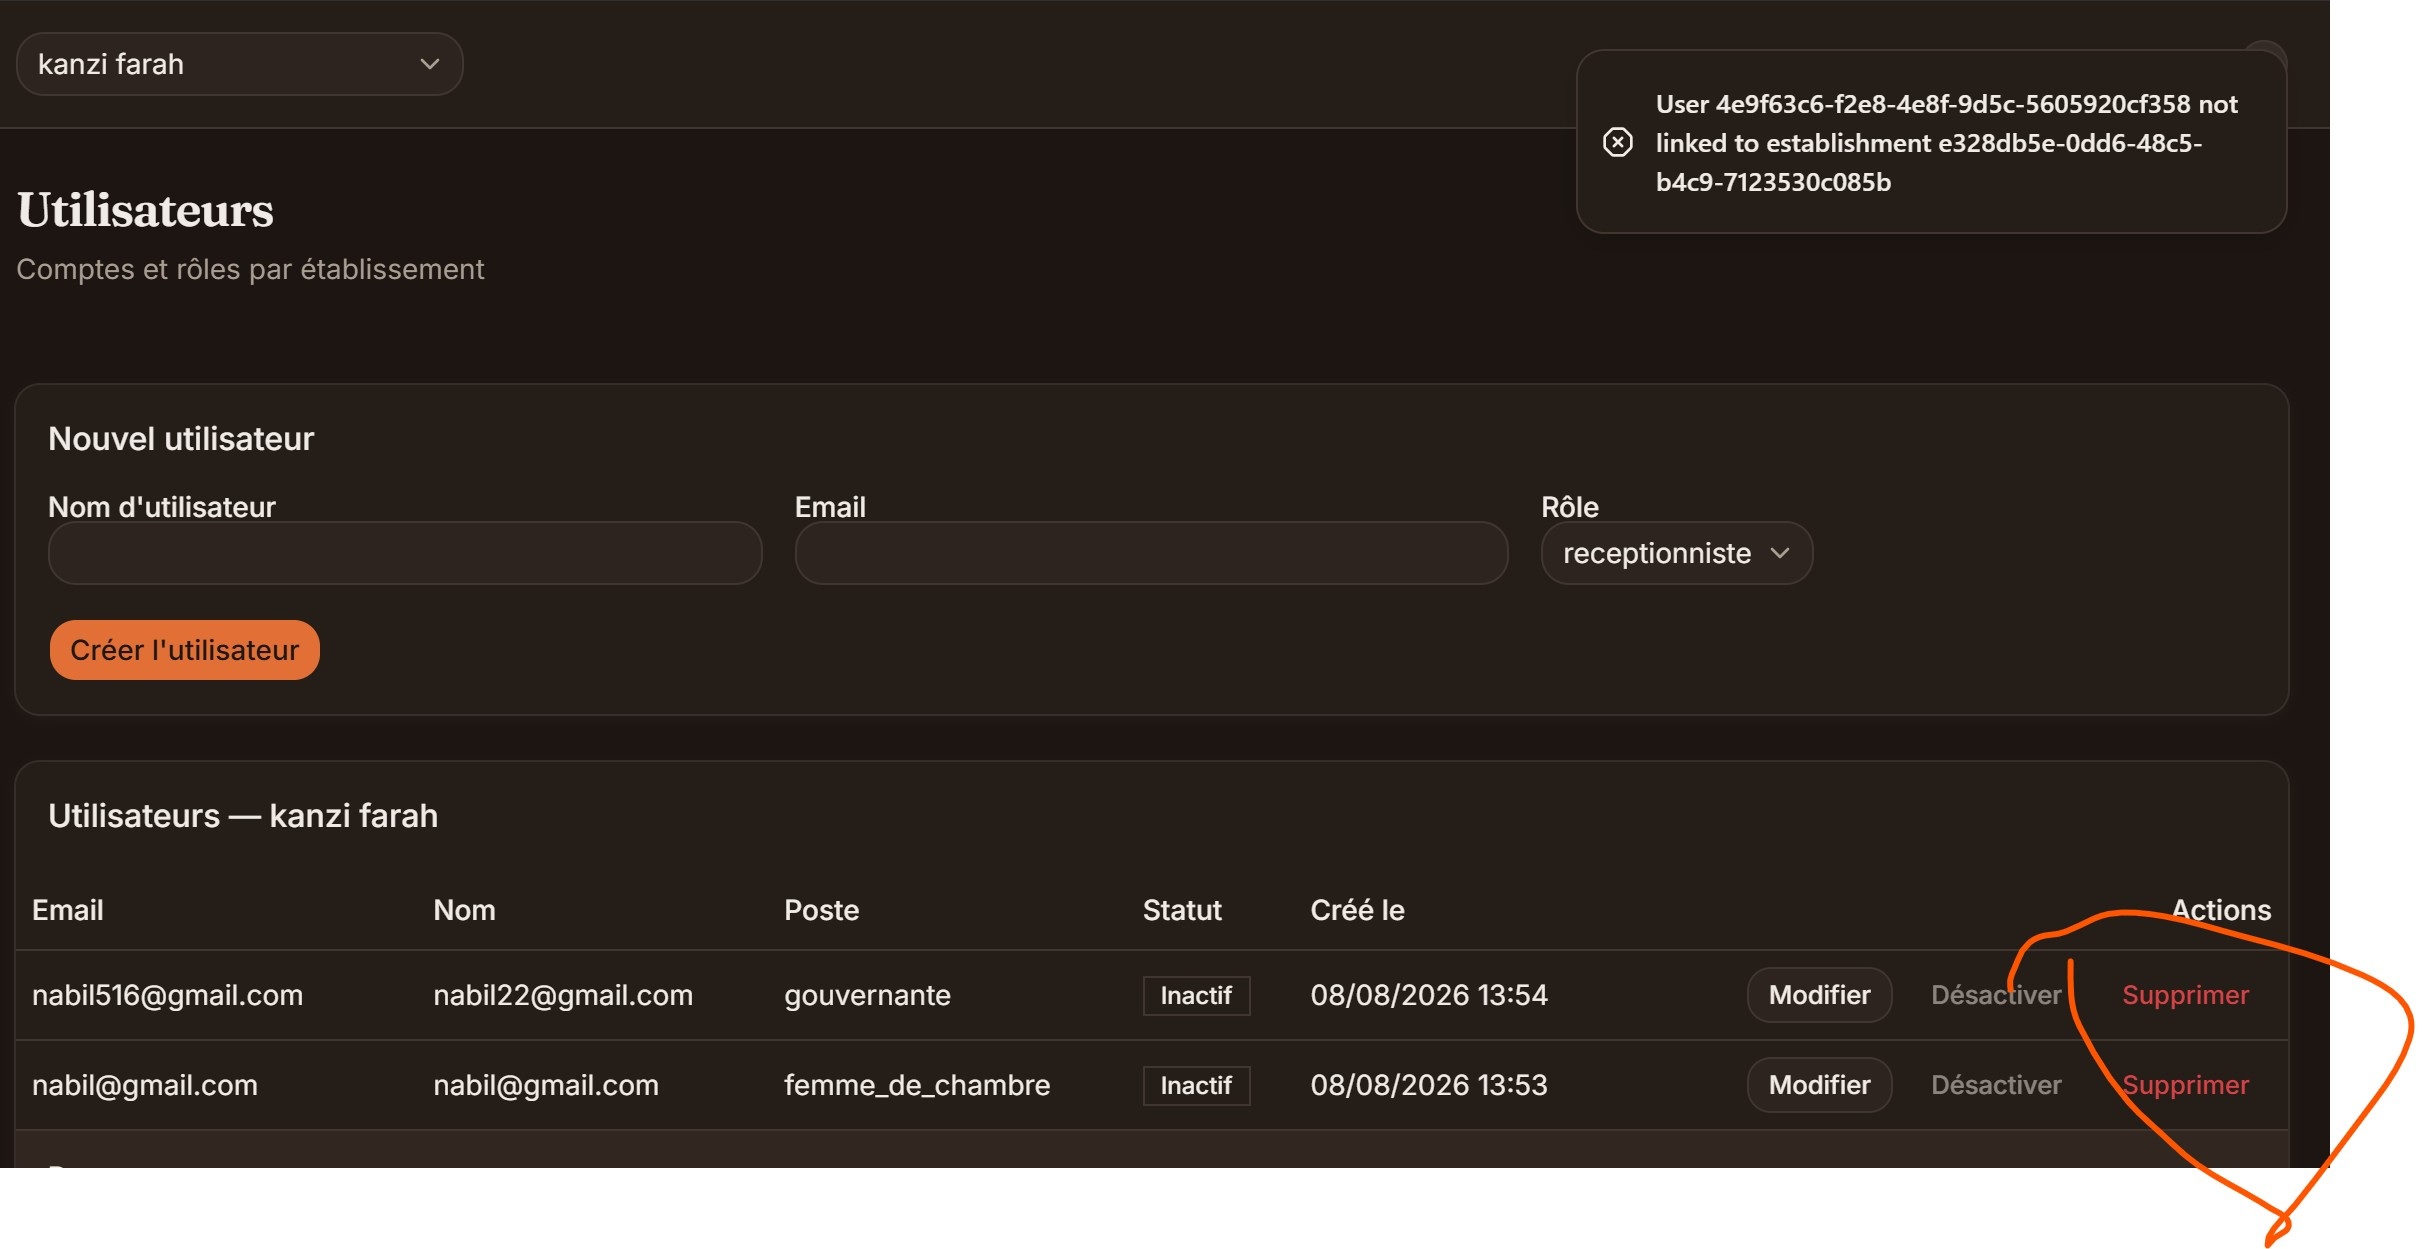
\includegraphics[width=0.75\textwidth]{figures/pic5.jpg}
\caption{Test d'ergonomie du planning Tape Chart sur poste de réception}
\label{fig:pic5}
\end{figure}

\begin{figure}[H]
\centering
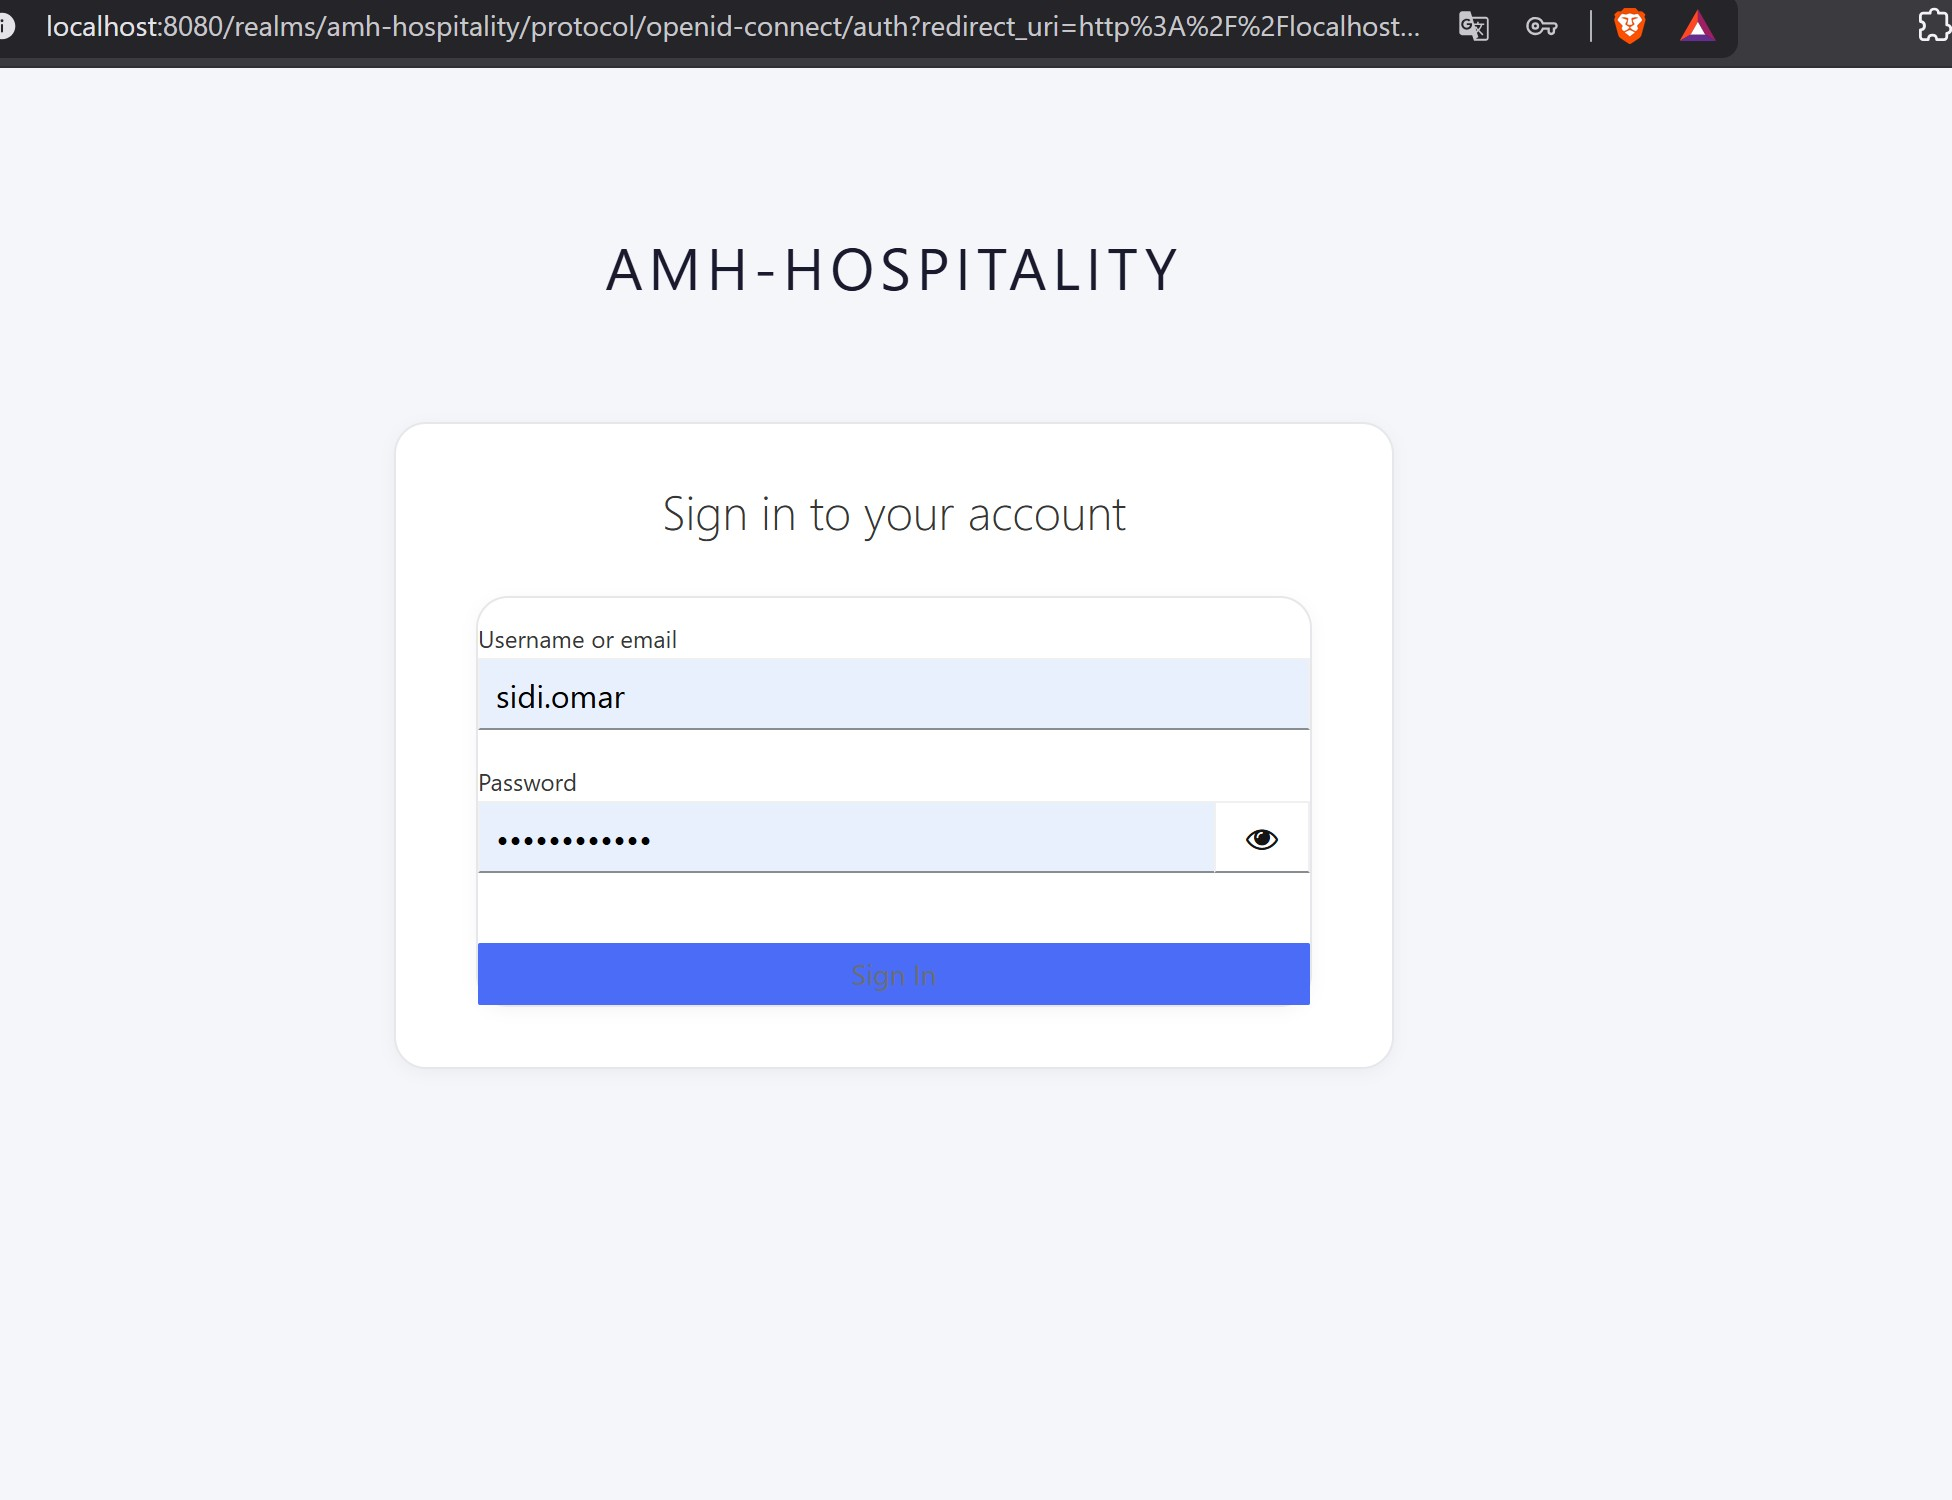
\includegraphics[width=0.75\textwidth]{figures/pic6.jpg}
\caption{Validation sur le terrain de la PWA mobile auprès du personnel d'étage}
\label{fig:pic6}
\end{figure}

Ces échanges réguliers sur le terrain ont constitué le garant indispensable de l'adéquation fonctionnelle et ergonomique de notre solution.

\subsection{Missions confiées}

Les missions confiées à notre équipe d'élèves-ingénieurs couvrent l'intégralité du cycle de vie du projet logiciel :
\begin{enumerate}
    \item \textbf{Audit et Analyse du Besoin} : Recueil des exigences fonctionnelles auprès des directeurs d'exploitation, réceptionnistes et gouvernantes ; formalisation du cahier des charges technique ;
    \item \textbf{Conception Architecturale} : Définition de l'architecture microservices selon les principes du \textit{Domain-Driven Design} (DDD) et du patron de conception \textit{Database per Service} ;
    \item \textbf{Développement Fullstack} : Implémentation des 11 microservices backend en Python (FastAPI), mise en place du serveur d'authentification centralisée (Keycloak) avec support WebAuthn/FIDO2, et développement de l'interface utilisateur moderne (Next.js 14, TypeScript, Tailwind CSS) ;
    \item \textbf{Assurance Qualité \& Tests} : Rédaction et exécution de tests unitaires (Pytest), d'intégration, de tests E2E, tests de charge et tests de vulnérabilités sécuritaires ;
    \item \textbf{Déploiement \& Observabilité} : Configuration de la passerelle d'API Kong, orchestration par Docker Compose, et audit continu sous SonarQube.
\end{enumerate}

\section{Présentation du projet PMS AMH Hospitality}

\subsection{Contexte et problématique détaillée}

Dans l'écosystème hôtelier moderne, le \textbf{PMS} (\textit{Property Management System}) constitue le véritable système nerveux central de l'établissement. Il pilote l'ensemble des flux opérationnels : de la première prise de contact du voyageur sur Internet jusqu'à son départ définitif, en passant par l'attribution de la chambre, la facturation des consommations au restaurant et la clôture financière nocturne.

Or, avant le lancement de notre projet, le groupe AMH Hospitality souffrait d'un environnement opérationnel fragmenté reposant sur des outils hétérogènes et des processus manuels lourds :

\begin{itemize}
    \item \textbf{Risques permanents de surréservation (\textit{Overbooking})} : Les disponibilités des chambres étaient mises à jour manuellement par les réceptionnistes sur les extranets des différentes OTA (Booking.com, Airbnb, Expedia). Ce décalage temporel créait des fenêtres de vulnérabilité où une même suite pouvait être louée simultanément sur deux canaux distincts, entraînant des litiges clients et des coûts exorbitants de relogement d'urgence dans des hôtels concurrents ;
    \item \textbf{Lourdeur critique du Night Audit manuel} : La procédure de clôture journalière exigeait de l'auditeur de nuit qu'il vérifie un à un tous les dossiers de séjours, recalcule manuellement les taxes de séjour et de promotion touristique, pointe les encaissements en espèces et cartes bancaires, et reporte à la main les soldes sur la journée suivante. Cette tâche fastidieuse mobilisait entre 1 heure et 2 heures chaque nuit, avec un risque élevé d'erreurs d'arrondis et d'asymétries d'écritures comptables ;
    \item \textbf{Failles de sécurité et d'imputabilité sur postes partagés} : Sur les banques de réception, les équipes se succédaient en utilisant des comptes génériques dotés de mots de passe partagés sur des post-it. En cas d'erreur de caisse, d'annulation frauduleuse ou de modification non autorisée de tarif, il était impossible d'imputer nominativement l'action à un opérateur précis ;
    \item \textbf{Défaut de synchronisation avec le service d'étage} : L'état d'entretien des chambres (sale, en cours de nettoyage, propre, inspectée) était communiqué par talkie-walkie ou sur feuilles volantes. Cette asynchronie provoquait de longs temps d'attente dans le patio pour les clients arrivant tôt (\textit{Early Check-in}), alors même que leur suite était déjà prête mais non signalée comme telle au système de réception ;
    \item \textbf{Cloisonnement des données entre établissements} : La direction générale ne disposait d'aucun tableau de bord consolidé pour piloter en temps réel les performances comparées des différents Riads du groupe.
\end{itemize}

\subsection{Objectifs stratégiques et opérationnels}

Pour résoudre définitivement l'ensemble de ces problématiques, notre projet s'est fixé les objectifs mesurables suivants :

\begin{itemize}
    \item \textbf{Zéro Overbooking} grâce à un mécanisme de verrouillage distribué temporaire sous Redis (TTL = 10 secondes) lors de la pose d'option de réservation ;
    \item \textbf{Clôture Night Audit en moins de 60 secondes} pour un parc de 50 chambres, entièrement automatisée et transactionnelle avec génération et archivage de rapports PDF immuables sur stockage MinIO S3 ;
    \item \textbf{Sécurité Zero-Trust et authentification biométrique WebAuthn/FIDO2} par QR code dynamique sur smartphone personnel, garantissant une traçabilité nominative à 100\% de chaque écriture financière ;
    \item \textbf{Application mobile PWA Housekeeping temps réel} connectée par WebSockets, réduisant le délai de mise à disposition des chambres propres à moins de 5 secondes après validation par la gouvernante ;
    \item \textbf{Architecture Multi-Tenant scalable} permettant d'embarquer de nouveaux Riads en moins de 10 minutes par simple configuration administrative sans modification de code source.
\end{itemize}

\section{Étude approfondie des besoins}

\subsection{Besoins fonctionnels par domaine métier}

Le Tableau~\ref{tab:besoins_f_detail} structure de manière exhaustive les exigences fonctionnelles attendues de la plateforme.

\begin{table}[H]
\centering
\small
\renewcommand{\arraystretch}{1.3}
\begin{tabularx}{\textwidth}{|p{3.8cm}|X|}
\hline
\textbf{Domaine Métier} & \textbf{Exigences et Fonctionnalités Détaillées} \\
\hline
\textbf{1. Authentification \& Sécurité (IAM)} & Authentification multifacteur : mot de passe fort + Passkey biométrique FIDO2 (TouchID/FaceID) via scan de QR code dynamique. Attribution des rôles RBAC (Super-Admin, Manager Riad, Réceptionniste, Gouvernante, Auditeur). Révocation instantanée des sessions actives. \\
\hline
\textbf{2. Planning Interactif (Tape Chart)} & Visualisation matricielle dynamique des chambres par catégorie et étage sur une échelle temporelle configurable. Création rapide de séjour par sélection de plage. Glisser-déposer (\textit{Drag \& Drop}) pour les changements de chambre (\textit{Room Shift}) avec recalcul instantané des écarts tarifaires. \\
\hline
\textbf{3. Moteur de Réservations} & Gestion du cycle de vie complet des réservations (Création, Confirmation, Modification, Annulation, No-Show). Verrouillage distribué Redis anti-collision. Support des réservations individuelles et de groupes multi-chambres. Gestion des canaux de distribution directs et OTA. \\
\hline
\textbf{4. Front Office (Arrivées / Départs)} & Processus de Check-in fluide avec vérification automatique du statut ménage propre. Saisie et validation des fiches d'identité et de police réglementaires. Attribution ou réaffectation de chambre. Processus de Check-out avec contrôle de solde nul obligatoire sur le folio. \\
\hline
\textbf{5. Facturation \& Folios Clients} & Création automatique d'un compte folio dès la réservation. Imputation automatique des nuitées d'hébergement. Imputation manuelle des extras (restaurant, spa, blanchisserie, excursions). Calcul automatique de la TVA (10\%) et des taxes marocaines (TS et TPT). Enregistrement multi-moyens de paiement (espèces, CB, virement) et génération de factures d'hébergement normalisées en PDF. \\
\hline
\textbf{6. Housekeeping (Gouvernance d'étage)} & Application mobile PWA ergonomique pour le personnel d'étage. Affichage des chambres assignées par statut (DIRTY, IN\_PROGRESS, CLEAN, INSPECTED, OUT\_OF\_ORDER). Mise à jour d'état en un clic avec diffusion immédiate par WebSockets vers le Tape Chart de réception. \\
\hline
\textbf{7. Clôture Nocturne (Night Audit)} & Module de clôture automatique contrôlant les départs et arrivées en suspens. Facturation en masse des nuitées et taxes de la date d'exploitation (\textit{Business Date}). Génération du rapport comptable journalier immuable archivé sur stockage S3 MinIO. Avancement atomique de la date d'exploitation (+1 jour). \\
\hline
\textbf{8. Administration Multi-Riads} & Gestion CRUD des établissements du groupe, des catégories de suites, des numéros de chambres, des équipements et des taux de taxes locales. Tableaux de bord de pilotage consolidés avec calcul automatique du RevPAR, de l'ADR et du taux d'occupation. \\
\hline
\end{tabularx}
\caption{Matrice détaillée des besoins fonctionnels du PMS AMH Hospitality}
\label{tab:besoins_f_detail}
\end{table}

\subsection{Besoins non fonctionnels}

Le Tableau~\ref{tab:besoins_nf_detail} formalise les exigences de qualité technique et d'exploitabilité industrielle.

\begin{table}[H]
\centering
\small
\renewcommand{\arraystretch}{1.3}
\begin{tabularx}{\textwidth}{|p{3.5cm}|X|}
\hline
\textbf{Catégorie de Qualité} & \textbf{Spécifications Techniques et Seuils d'Acceptation} \\
\hline
\textbf{Performance \& Latence} & Temps de réponse des API REST inférieur à 200 ms pour 95\% des requêtes ($p95$). Clôture Night Audit complète exécutée en moins de 60 secondes pour 50 chambres. Chargement initial du Tape Chart en moins de 1.2 seconde. \\
\hline
\textbf{Sécurité \& Confidentialité} & Chiffrement SSL/TLS (HTTPS) de tous les flux réseau. Signature asymétrique RS256 des jetons JWT. Mots de passe hachés sous Argon2id. Isolation stricte des données entre locataires (\textit{Multi-Tenancy}). Conformité à la loi marocaine 09-08 et au RGPD. \\
\hline
\textbf{Disponibilité \& Résilience} & Architecture microservices conteneurisée tolérante aux pannes : l'indisponibilité du service Housekeeping n'interrompt pas les fonctions de réservation du Front Office. \\
\hline
\textbf{Cohérence Transactionnelle} & Propriétés ACID strictes sur l'ensemble des opérations financières et comptables sous PostgreSQL. Gestion de l'exclusion mutuelle par verrous Redis. \\
\hline
\textbf{Ergonomie \& Responsive} & Interface web moderne avec feedbacks visuels immédiats (toasts d'alerte, barres de progression). PWA mobile optimisée pour les écrans tactiles des gouvernantes. \\
\hline
\textbf{Maintenabilité \& Testabilité} & Code structuré selon le Domain-Driven Design. Taux de couverture de tests unitaires automatisés supérieur à 80\%. Analyse statique SonarQube avec Quality Gate Passed (Note A). \\
\hline
\end{tabularx}
\caption{Spécifications détaillées des exigences non fonctionnelles}
\label{tab:besoins_nf_detail}
\end{table}

\section{Conduite du projet selon la méthode Agile Scrum}

\subsection{Principes et justification de la méthode Scrum}

La Figure~\ref{fig:logo_scrum} et la Figure~\ref{fig:scrum_flow} illustrent le cadre méthodologique Agile Scrum adopté pour structurer le cycle de développement du projet.

\begin{figure}[H]
\centering
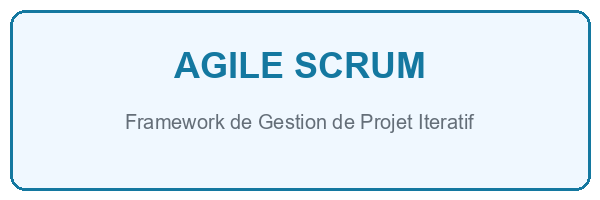
\includegraphics[width=0.5\textwidth]{figures/logo_scrum.png}
\caption{Logo du framework Agile Scrum}
\label{fig:logo_scrum}
\end{figure}

\begin{figure}[H]
\centering
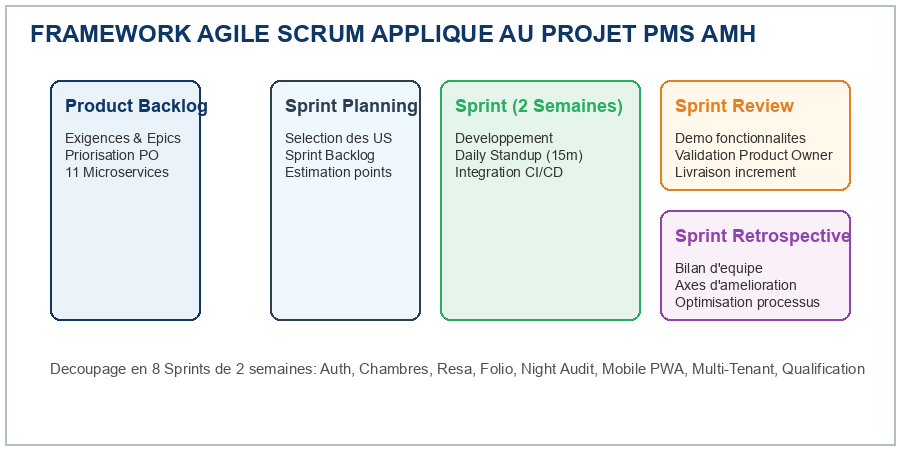
\includegraphics[width=0.85\textwidth]{figures/scrum_framework.png}
\caption{Organisation du cycle de développement Scrum appliqué au PMS AMH}
\label{fig:scrum_flow}
\end{figure}

Le choix du framework Agile Scrum s'est imposé en raison de la nature itérative du projet et de la nécessité de confronter régulièrement les fonctionnalités développées aux retours d'expérience des équipes opérationnelles des Riads. Scrum repose sur des itérations à durée fixe appelées \textbf{sprints} (ici fixés à 2 semaines), au terme desquels un incrément logiciel fonctionnel, testé et potentiellement livrable est produit.

L'organisation de notre équipe Scrum a été définie comme suit :
\begin{itemize}
    \item \textbf{Product Owner (PO)} : Notre encadrant professionnel (Lead Architect), représentant les besoins des directeurs de Riads, garant de la vision produit et responsable de la priorisation du Product Backlog ;
    \item \textbf{Scrum Master (SM)} : Rôle assuré par rotation entre les membres de notre équipe, veillant au respect des cérémonies agiles et à la levée rapide des obstacles techniques ;
    \item \textbf{Équipe de Développement (Dev Team)} : Les trois élèves-ingénieurs (Nabil BOUDARINE, Youssef OUIZZA, Hamza IBN TALIB), assurant de manière collective et pluridisciplinaire la conception, l'implémentation backend et frontend, les tests et le déploiement.
\end{itemize}

Les cérémonies Scrum appliquées durant les 16 semaines du projet ont inclus :
\begin{itemize}
    \item \textbf{Sprint Planning} (en début de chaque quinzaine) : Sélection des User Stories du Product Backlog à intégrer dans le Sprint Backlog et estimation de l'effort en points de complexité (Planning Poker) ;
    \item \textbf{Daily Scrum} (chaque matin, 15 minutes) : Synchronisation de l'équipe autour des trois questions rituelles : ce qui a été réalisé la veille, les tâches du jour et les éventuels blocages rencontrés ;
    \item \textbf{Sprint Review} (en fin de quinzaine) : Démonstration en direct de l'incrément réalisé devant le Product Owner et les réceptionnistes référents pour validation formelle ;
    \item \textbf{Sprint Retrospective} : Analyse critique du fonctionnement interne de l'équipe pour identifier les axes d'amélioration technique et organisationnelle pour le sprint suivant.
\end{itemize}

\subsection{Découpage des sprints et livrables}

Le projet a été structuré en huit sprints thématiques de deux semaines, tel que décrit dans le Tableau~\ref{tab:sprints_detail}.

\begin{table}[H]
\centering
\small
\renewcommand{\arraystretch}{1.3}
\begin{tabularx}{\textwidth}{|p{2.2cm}|p{3.2cm}|X|}
\hline
\textbf{Sprint} & \textbf{Période Calendaire} & \textbf{Objectifs, Réalisations et Livrables Clés} \\
\hline
\textbf{Sprint 1} & Semaines 1--2 & Cadrage général, immersion en Riad, audit de l'existant, Product Backlog initial. Mise en place du monorepo GitHub, du pipeline CI/CD de base et de l'environnement Docker Compose. \\
\hline
\textbf{Sprint 2} & Semaines 3--4 & Déploiement de la passerelle Kong API Gateway. Configuration du serveur d'identité Keycloak (OIDC, RBAC). Implémentation du service Auth FastAPI et de l'authentification biométrique WebAuthn/FIDO2 avec flux QR Code. \\
\hline
\textbf{Sprint 3} & Semaines 5--6 & Développement du service Référentiel des Établissements (Riads, catégories, chambres, taxes). Développement du service Réservation avec moteur de verrouillage distribué anti-collision sous Redis. \\
\hline
\textbf{Sprint 4} & Semaines 7--8 & Développement du service Gestion des Clients (Guest Profile). Implémentation frontend du planning matriciel interactif Tape Chart sous Next.js 14 avec Drag \& Drop et gestion des changements de chambre (\textit{Room Shift}). \\
\hline
\textbf{Sprint 5} & Semaines 9--10 & Développement du module Front Office (Check-in, Check-out, fiches de police). Développement du service Facturation et Folios (création de comptes, imputation des charges et extras, calcul des soldes). \\
\hline
\textbf{Sprint 6} & Semaines 11--12 & Implémentation des moteurs de calcul fiscal marocain (TVA 10\%, TS 25 MAD, TPT 12 MAD). Développement du moteur de Night Audit automatisé transactionnel avec génération de rapports PDF et archivage MinIO S3. \\
\hline
\textbf{Sprint 7} & Semaines 13--14 & Développement de l'application mobile progressive (PWA) Housekeeping pour le personnel d'étage. Implémentation de la diffusion temps réel WebSockets et du centre de notifications via RabbitMQ. \\
\hline
\textbf{Sprint 8} & Semaines 15--16 & Campagnes de tests de charge et de performance (15 utilisateurs concurrents). Audit statique de code sous SonarQube avec Quality Gate Passed. Qualification finale, validation sur site pilote et rédaction du mémoire. \\
\hline
\end{tabularx}
\caption{Découpage des sprints Scrum et livrables associés}
\label{tab:sprints_detail}
\end{table}

\subsection{Planification temporelle par diagramme de Gantt}

La Figure~\ref{fig:gantt_pms} présente le diagramme de Gantt illustrant l'ordonnancement séquentiel et les dépendances entre les différentes phases du projet sur l'ensemble des 16 semaines de réalisation.

\begin{figure}[H]
\centering
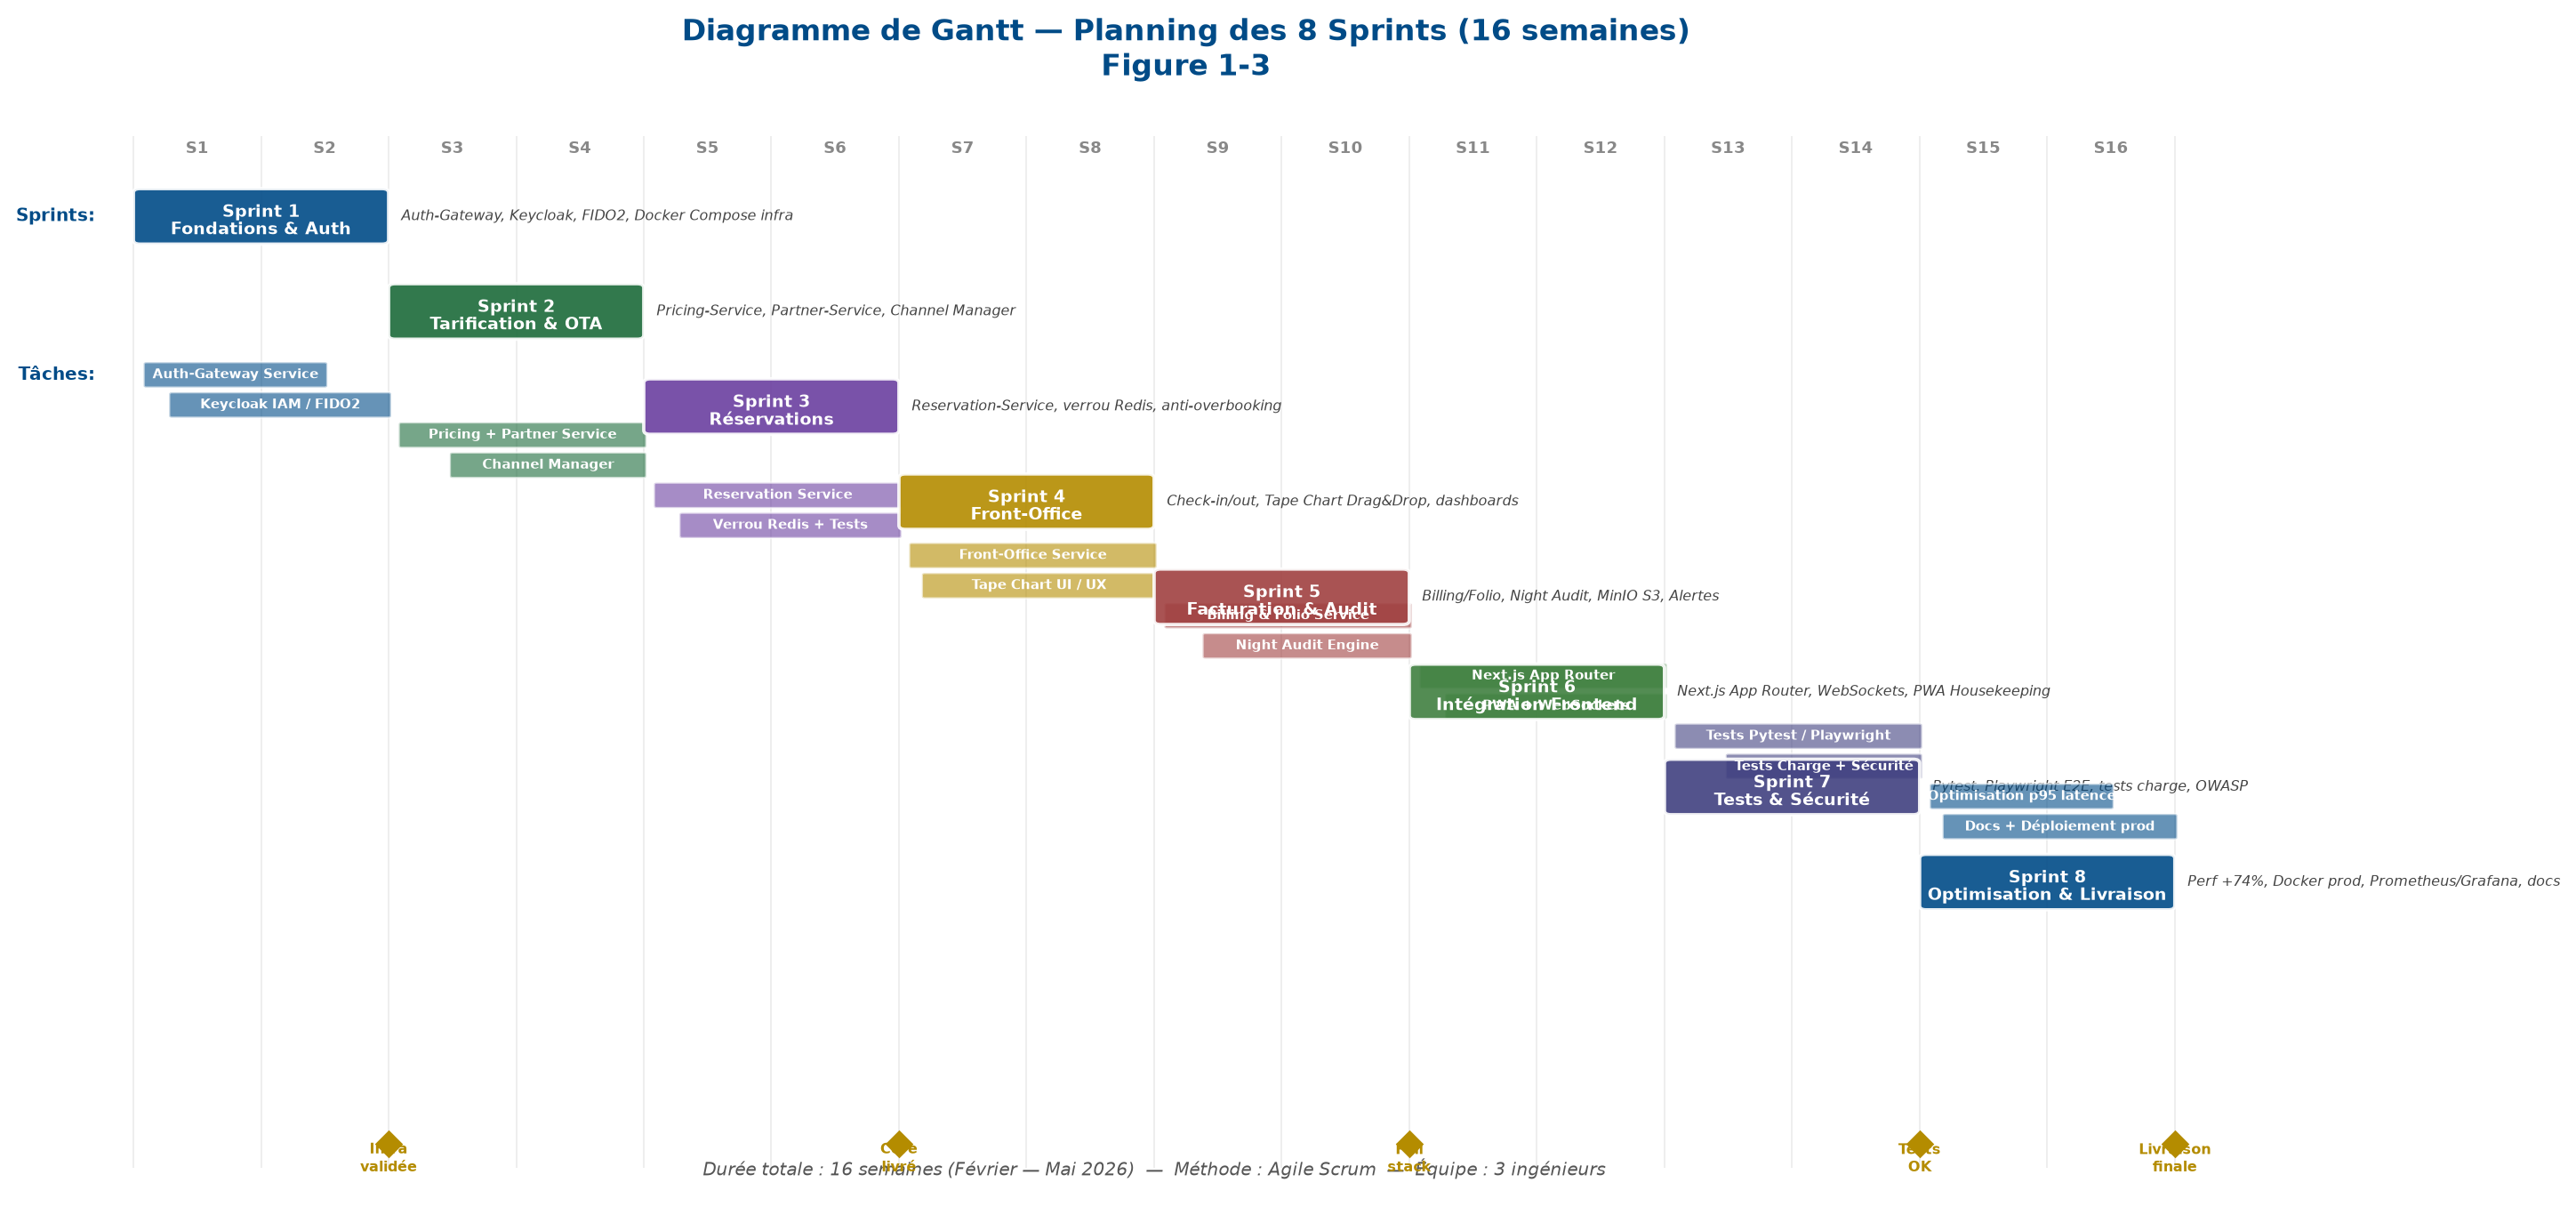
\includegraphics[width=0.95\textwidth]{figures/gantt_pms.png}
\caption{Diagramme de Gantt de la planification temporelle du projet}
\label{fig:gantt_pms}
\end{figure}

\section{Conclusion}

Ce premier chapitre a posé les bases contextuelles, industrielles et méthodologiques de notre projet de fin d'année. Nous avons présenté le groupe AMH Hospitality, analysé en profondeur les dysfonctionnements structurels de la gestion traditionnelle des Riads à Marrakech, et défini les objectifs techniques majeurs de la plateforme logicielle. L'étude détaillée des exigences et l'organisation du projet selon le framework Agile Scrum ont constitué le cadre de travail rigoureux ayant guidé notre équipe. Le chapitre suivant sera consacré à l'analyse formelle des besoins et à la modélisation conceptuelle et structurelle du système à l'aide du standard UML.
